\graphicspath{{images/}}

\section{\thesection~Methods}
\label{sec:methods}

\subsection{\thesubsection~Conversion between models}

The reaction equation of the competition model \ref{eq:reaction}
assumes that all nutrients are converted to cells. This implies that
cultures starting with the same amount of nutrients reach the same
final amount of cells. (Discussion: The identity of the nutrient
molecule is unknown and it is not clear whether metabolism of the
nutrient molecule will have a significant effect. If necessary a
metabolism reaction could also be modelled.) To fit the mass action
kinetic logistic model, it is necessary to assume different
\(N_{t_{0}}\) for each culture which is not physical.



\begin{Figure}
  \centering
  \graphicspath{{images/correction/}}
  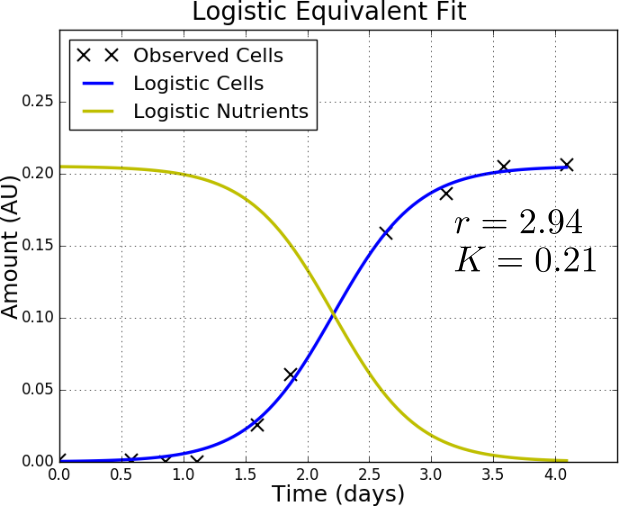
\includegraphics[width=\linewidth]{final/logistic}
  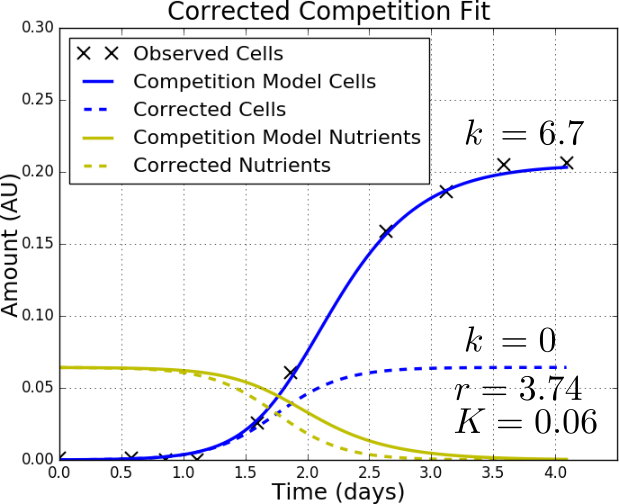
\includegraphics[width=\linewidth]{final/competition}
  \captionof{figure}{\textbf{Using the competition model to correct
      for competition.} Fits are to culture (R10, C3) of P15 which
    grew faster and reached a higher final cell density than its
    neighbours (not shown). According to the competition model, this
    is because this culture competed for more nutrients. To reach the
    same final cell density, the logistic equivalent model requires a
    higher amount of starting nutrients for this culture and a
    different amount for each neighbour. The correction to the
    competition model simulates how growth would have appeared without
    competition and allows us to return parameters \(r\) and \(K\) of
    the logistic model.}
  \label{fig:correction}
\end{Figure}

%%% Local Variables:
%%% mode: latex
%%% TeX-master: "report"
%%% End:
